The fifth question of the survey asked the participants whether they follow SOLID principles while developing Android applications. Results have shown that 66.3\% of the participants declared that they follow SOLID principles and 20.6\% of them declared that they might follow these principles. 6.3\% of the participants stated that they do not apply the SOLID principles, and 6.9\% stated that they are not aware of these principles. The figure below contains the graphical breakdown of this data.
\begin{figure}[ht!]
    \centering
    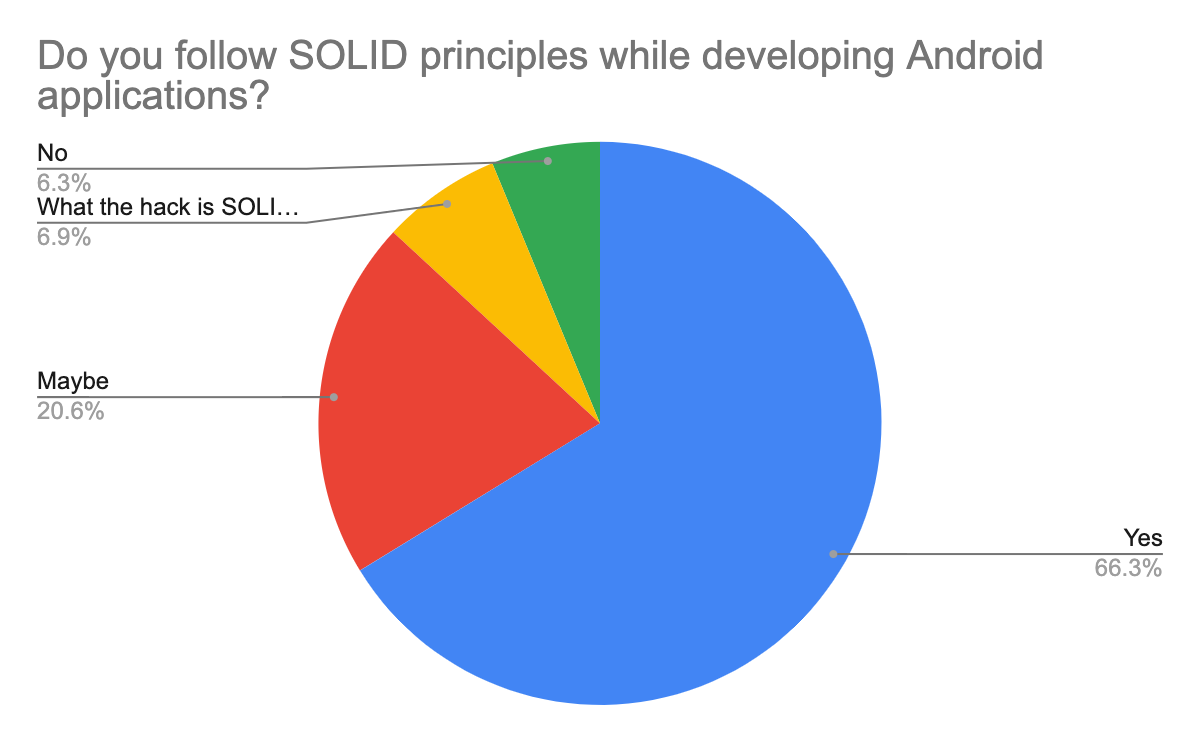
\includegraphics[scale=0.22]{figures/survey_q5_solid.png}
    \caption{SOLID principles usage results}
    \label{fig:solid}
\end{figure}
\FloatBarrier

The 6th question of the survey asks the participants whether they apply the "Clean Code" principles while developing Android applications. The results in the form of a pie chart can be seen below in Fig. \ref{fig:clean_code}.
\begin{figure}[ht!]
    \centering
    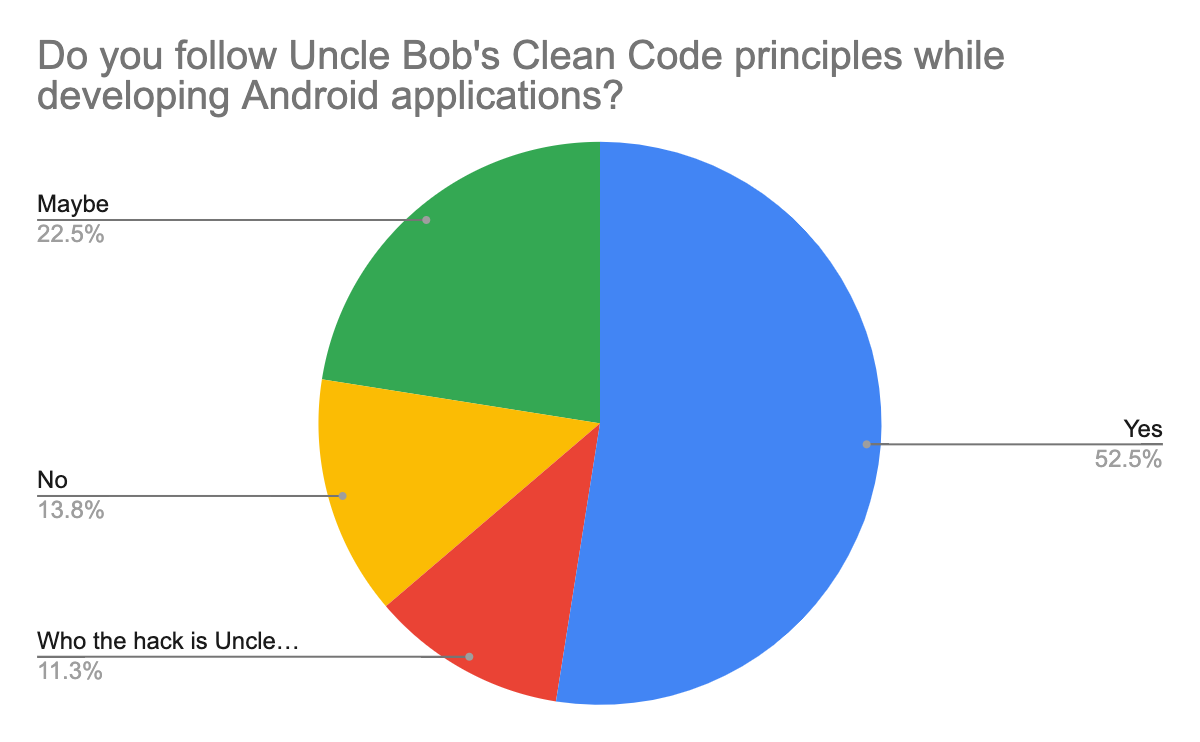
\includegraphics[scale=0.22]{figures/survey_q6_clean_code.png}
    \caption{Clean Code principles usage results.}
    \label{fig:clean_code}
\end{figure}
\FloatBarrier

According to the results, 75\% of the participants stated that they either used or could use these principles. While 13.8\% of the participants stated that they do not use these principles, it was observed that 11.3\% of the participants were not even aware of these principles.
